	%%%
	%%% V7
	%%%

	\subsection{Polymorphismus in Haskell} % (fold)
	\label{sub:polymorphismus_in_haskell}
		\begin{itemize}
			\item parametrischen über Typvariablen\\
			(Im Tysp dürfen Typfedinitionen auftauchen)
			\item ad-hoc übr Typklassen
		\end{itemize}

		\subsubsection*{Unterschied} % (fold)
		\label{ssub:unterschied}
			\begin{tabular}{lcp{8cm}}
				ad-hoc & $\equiv$ & derselbe Name für unterschiedliche Algorithmen\\
				parametrischer & $\equiv$ & derselbe Name für den gleichen Algorithmus, also ein Algorithmus für alle Typen
			\end{tabular}
		% subsubsection unterschied (end)

		% subsubsection beispiel_parametrischer_polymorphismus (end)
	% subsection polymorphismus_in_haskell (end)
		\subsubsection*{Beispiel ad-hoc Polymorphismus} % (fold)
		\label{ssub:beispiel_ad_hoc_polymorphismus}
					\lstHaskell
			\begin{lstlisting}
show
			\end{lstlisting}
	\subsection{Weltveränderung} % (fold)
	\label{sub:weltveraenderung}
		\lstHaskell
		\begin{lstlisting}[morekeywords={sgetLine}]
sgetLine :: IO String
		\end{lstlisting}
		\lstHaskell
		\begin{lstlisting}
p :: IO a
q :: IO b
p >> q :: IO b
p >> q = \w -> let (a,w') = p w
                   (b,w'') = q w'
               in (b,w'')
		\end{lstlisting}
		Was nichts anderes ist als
		\lstHaskell
		\begin{lstlisting}
p >> q = q.snd.p
		\end{lstlisting}
		\lstHaskell
		\begin{lstlisting}
getChar :: IO Char
putChar :: Char -> IO ()
		\end{lstlisting}
		\lstHaskell
		\begin{lstlisting}
(>>=) :: IO a -> (a -> IO b) -> IO b
p :: IO a
f :: a -> IO a

p >>= f :: IO b
p >>= f = \w -> let (a,w') = p w
                    (b,w'') = w'
                in (b,w'')
		\end{lstlisting}
				Haskell setzt um:
		\lstHaskell
		\begin{lstlisting}
do {a; b} == do a
                b
do{a}=a
do{a;as}=a>>(do{as})
do{v<-a,as}=a>>=(\v->do{as})
		\end{lstlisting}

		\lstHaskell
		\begin{lstlisting}
{f;g;}h; != f;{g;h;}
		\end{lstlisting}
		\lstHaskell
		\begin{lstlisting}
data Ampel = Rot
           | Gelb
           | Gruen
data Tree a = Nil |
              Node a Tree Tree
		\end{lstlisting}
		\lstHaskell
		\begin{lstlisting}
IO (\w -> ((),w)) == IO $ \w -> ((),w)
		\end{lstlisting}

		%%%
		%%% end V7
		%%%
		%%%
		%%% V8
		%%%

		\lstHaskell
		\begin{lstlisting}
-- generisch
MState s a

-- konkret
MS (\x -> (x,17))

-- und damit Typ
MState s Int
		\end{lstlisting}

		\lstHaskell
		\begin{lstlisting}
bla = MS (\x -> (x,17))
(runMState bla) :: s -> (s,Int)
		\end{lstlisting}

		\lstHaskell[Mitzählen von \texttt{getc} als Aktion, aber keine Auslieferung]
		\begin{lstlisting}
getc = \s -> (s+1,s)
		\end{lstlisting}

		\lstHaskell[Zähler zurücksetzen]
		\begin{lstlisting}
put = \s' -> MS $ \s -> (s',s)
		\end{lstlisting}

		\lstHaskell[Kurzform vereinfacht Nutzung und Schachtelung]
		\begin{lstlisting}
-- Langform
MState s a

-- Kurzform
m a

-- Nutzung
instance Monad m where
		\end{lstlisting}

		\lstHaskell[detaillierte Aufschlüsselung anhand von \texttt{get >>= put}]
		\begin{lstlisting}
get = MS (\s -> (s,s))
put = \s' -> MS (\s -> (s',s))
runMState (MS f) = f

get >>= put

MS (\s -> let (s',a) = runMState (MS (\s -> (s,s))) s
          in runMState (put s) s')
MS (\s -> let (s',a) = (\s -> (s,s)) s
          in runMState (put s) s')
MS (\s -> let (s',a) = (s,s)
          in runMState (put s) s')
MS (\s -> runMState (put s) s)
MS (\s -> runMState (MS (\s -> (s,s))) s)
MS (\s -> (\s -> (s,s)) s)
MS (\s -> (s,s))
		\end{lstlisting}
		get $>>=$put
		\begin{itemize}
			\item nimmt den aktuellen Zustand raus als Ergebnis
			\item fügt den Zustand als Argument in den Input
			\item Verändert den Zustand nicht und liefert ihn als Ergebnis
		\end{itemize}
		
		\begin{figure}[ht]
			\caption{Realisierung Verkettung äußerer mit innerer Monade}
			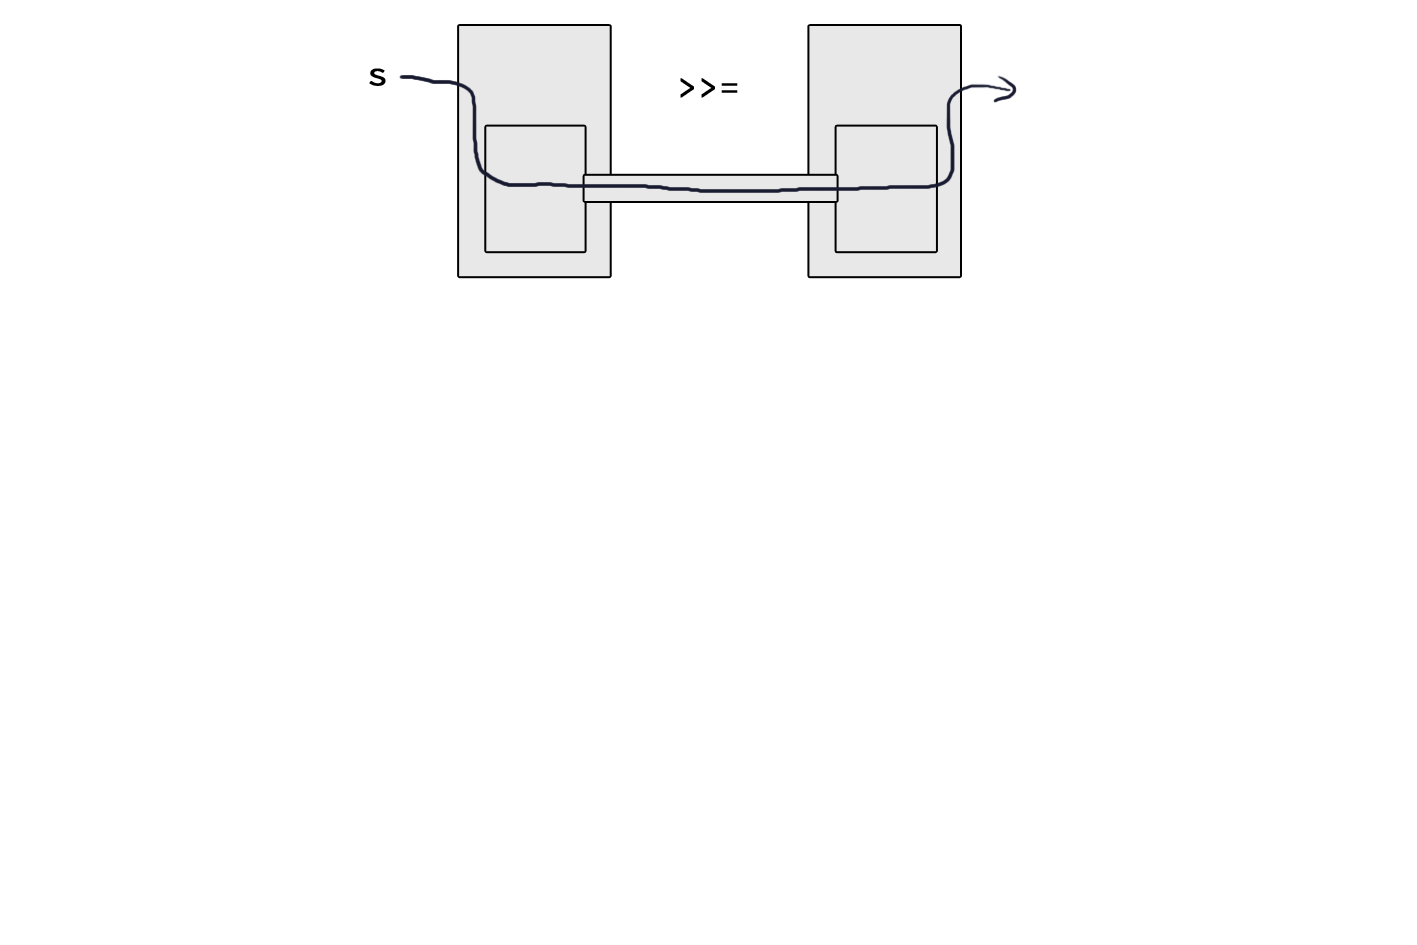
\includegraphics[width=\textwidth]{workfiles/v8_1}
		\end{figure}
	% subsection weltveraenderung (end)

	%%%
	%%% end V8
	%%%

	%%%
	%%% V9
	%%%

	\newpage
	\subsection{Detailliertes Herleitungsbeispiel} % (fold)
	\label{sub:detailliertes_herleitungsbeispiel}
	
		\lstHaskell[allgemeine Monade]
		\begin{lstlisting}
type IO a = World -> (World,a)
		\end{lstlisting}

		\lstHaskell[Welt mit einer Int-Zahl]
		\begin{lstlisting}
type IntW = (Int, World)
		\end{lstlisting}

		\lstHaskell[Monade mit dieser Welt]
		\begin{lstlisting}
type IIO a = IntW -> (IntW,a)
		\end{lstlisting}

		\subsubsection{Inkrement} % (fold)
		\label{ssub:inkrement}
		
			\lstHaskell
			\begin{lstlisting}
inc :: IIO Int -- Rueckgabe Int beliebig
inc = \(i,w) -> ((i+1,w),i)
			\end{lstlisting}

		% subsubsection inkrement (end)

		\subsubsection{putString} % (fold)
		\label{ssub:putstring}
		
			\lstHaskell
			\begin{lstlisting}
putStrI :: String -> IIO ()
putStr :: String IO ()
putStrI = \s -> \(i,w) -> let (w',a) = putStr s w
                          in ((i+1,w'),a)
			\end{lstlisting}

		% subsubsection putstring (end)

		\subsubsection{Problem der unerreichbaren Welt} % (fold)
		\label{ssub:problem_der_unerreichbaren_welt}

			Problem: Kommen nicht an \texttt{w} heran\\
			Ziel: Eleminierung von \texttt{w} als Argument, kennen wir bereits von der Verkettung:

			\begin{flalign*}
(f\circ g) (x) = f(g(x))
			\end{flalign*}

			\lstHaskell[vom Mathematischen zum Quellcode]
			\begin{lstlisting}[mathescape]
pq = \x -> p(q(x))
pq = p $\circ$ q -- pointless function definition
			\end{lstlisting}

			\lstHaskell[Umbauen]
			\begin{lstlisting}
type IIO a = (Int,World) -> ((Int,World),a)
           = Int -> World -> ((Int,World),a) -- Curryfizierung
           = Int -> World -> (World,(Int,a)) -- Umsortierung
           = Int -> IO (Int,a)
			\end{lstlisting}
		
		% subsubsection problem_der_unerreichbaren_welt (end)

		\subsubsection{return} % (fold)
		\label{ssub:return}

			\lstHaskell
			\begin{lstlisting}
return :: a -> IO a
return i = \w -> (w,i)
			\end{lstlisting}
		(ermöglicht es Nutzern von return, die Welt w weg zu lassen)
		% subsubsection return (end)

		\subsubsection{Inkrement, neu} % (fold)
		\label{ssub:inkrement_neu}
		
			\lstHaskell
			\begin{lstlisting}
inc :: IIO Int
inc :: Int -> World -> (World,(Int,Int))
inc i w = (w,(i+1,i+1))
inc i = \w -> (w,(i+1,i+1))
--      :: IO (Int,Int)
      = return (i+1,i+1)
			\end{lstlisting}

		% subsubsection inkrement_neu (end)

		\subsubsection{putStrI, neu} % (fold)
		\label{ssub:putstri_neu}
		
			\lstHaskell
			\lstset{
				moredelim=**[is][{\btHL[p]}]{@}{@},
				moredelim=**[is][{\bbHL[f]}]{_}{_},
			}
			\begin{lstlisting}
putStrI :: String -> IIO ()
putStrI :: String -> Int -> World -> (World,(Int,()))
putStrI s = \i -> \w -> let (w',a) = putStr s w
                        in (w',(i+1,a))
putStrI s = \i -> \w -> let (w',a) = putStr s w
                        in return (i+1,a) w'
putStrI s = \i -> \w -> let (w',a) = @putStr s@ w
                        in _(\x -> return (i+1,x))_ a w'
putStrI s = \i -> outStr s >>= (\x -> return (i+1,x))
			\end{lstlisting}

		% subsubsection putstri_neu (end)

		\subsubsection{Verkettung} % (fold)
		\label{ssub:verkettung}
		
			\lstHaskell
			\lstset{
				moredelim=**[is][{\btHL[p]}]{@}{@},
				moredelim=**[is][{\bbHL[f]}]{_}{_},
			}
			\begin{lstlisting}
(>>) :: IIO a -> IIO b -> IIO b
ia >> ib = \i -> \w = let (w',ria) = @ia i@ w
                      in _ib_ ria w'
ia >> ib = \i -> ia >>= ib
			\end{lstlisting}

		% subsubsection verkettung (end)

		\subsubsection{Verfeinerung Typdefinition} % (fold)
		\label{ssub:verfeinerung_typdefinition}
		
			\lstHaskell
			\begin{lstlisting}
type IIO a = Int -> IO (Int,a)
type IIO s a = s -> IO (s,a)
type IIO s m a = s -> m (s,a)
type ST s m a = s -> m (s,a)
			\end{lstlisting}

		% subsubsection verfeinerung_typdefinition (end)

		\subsubsection{putStrt} % (fold)
		\label{ssub:putstrt}
		
			\lstHaskell
			\begin{lstlisting}
putStrt :: StateT Int IO a
putStrt = liftST putStr
          liftST (putStr " ") >> liftST (print)
			\end{lstlisting}

		% subsubsection putstrt (end)

	% subsection detailliertes_herleitungsbeispiel (end)

	%%%
	%%% end V9
	%%%

	%%%
	%%% V10
	%%%

	Wir haben

	\lstHaskell
	\begin{lstlisting}
(StateT s m) a
(MaybeT m) a
	\end{lstlisting}

	wollen nun IO-Monaden erweitern, um auch Berechnung abbrechen zu können

	\lstHaskell
			\lstset{
				moredelim=**[is][{\bbHL[Monade]}]{_}{_},
				moredelim=**[is][{\bbHL[Monade]}]{@}{@},
			}
	\begin{lstlisting}
@MaybeT _(StateT s IO)_@ a
	\end{lstlisting}